\documentclass[titlepage,a4paper]{article}

\usepackage{a4wide}
\usepackage[colorlinks=true,linkcolor=black,urlcolor=blue,bookmarksopen=true]{hyperref}
\usepackage{bookmark}
\usepackage{fancyhdr}
\usepackage[spanish]{babel}
\usepackage[utf8]{inputenc}
\usepackage[T1]{fontenc}
\usepackage{graphicx}
\usepackage{float}
\usepackage[margin=0.65in]{geometry}
\usepackage[spanish]{babel}
\usepackage{listings}
\usepackage{xcolor}
\usepackage{longtable}

\pagestyle{fancy} % Encabezado y pie de página
\fancyhf{}
\fancyhead[L]{TP Diseño - Coffee Shop Analysis}
\fancyhead[R]{Sistemas Distribuidos I - FIUBA}
\renewcommand{\headrulewidth}{0.4pt}
\fancyfoot[C]{\thepage}
\renewcommand{\footrulewidth}{0.4pt}

\begin{document}
\begin{titlepage} % Carátula
	\hfill
\includegraphics[width=6cm]{logofiuba.jpg}
    \centering
    \vfill
    \Huge \textbf{TP Diseño - Coffee Shop Analysis}
    \vskip2cm
    \Large [75.74] Sistemas Distribuidos I\\
    Segundo cuatrimestre de 2025 
    \vfill
    \begin{tabular}{ | l | l | l |}
      \hline
      Avecilla, Ignacio & 105067& iavecilla@fi.uba.ar\\ \hline
      Avila, Gaston& 104482& gavila@fi.uba.ar\\ \hline
      Muñoz, Juan Martín & 106699& jmmunoz@fi.uba.ar\\ \hline
  	\end{tabular}
    \vfill
    \vfill
\end{titlepage}

\tableofcontents % Índice general
\newpage

\section{Alcance}\label{sec:alcance}
\paragraph{El presente informe presenta la documentación de un sistema distribuido flexible, robusto y escalable, capaz de resolver las consultas otorgadas por la catedra con una cantidad de unidades de procesamiento mayor o igual a uno.}

\paragraph{Las consultas a resolver son:}
\begin{enumerate}
    \item Transacciones (Id y monto) realizadas durante 2024 y 2025 entre las 06:00 AM y las
11:00 PM con monto total mayor o igual a 75.
\item Productos más vendidos (nombre y cant) y productos que más ganancias han generado
(nombre y monto), para cada mes en 2024 y 2025.
\item TPV (Total Payment Value) por cada semestre en 2024 y 2025, para cada sucursal, para
transacciones realizadas entre las 06:00 AM y las 11:00 PM.
\item Fecha de cumpleaños de los 3 clientes que han hecho más compras durante 2024 y
2025, para cada sucursal.
\end{enumerate}

\section{Arquitectura}\label{sec:arquitectura}

\subsection{Vista Física}
\paragraph{Se muestra la enteridad del sistema y las conexiones existentes entre las diversas entidades del sistema.}

\subsubsection{Diagrama de Robustez}
\paragraph{Se visualizan todos los componentes que interactuan en nuestro diseño, desde la interacción inicial del cliente, hasta la finalización del procesado de todas las consultas.}
\begin{itemize}
    \item Los trabajadores se comunican a través de la inserción y consumo de datos en diversas colas, las cuales pueden ser accedidas por multiples trabajadores concurrentemente. Se distinguen 2 tipos de cola segun como se distribuyen los mensajes:
\begin{figure}[H]
\centering
    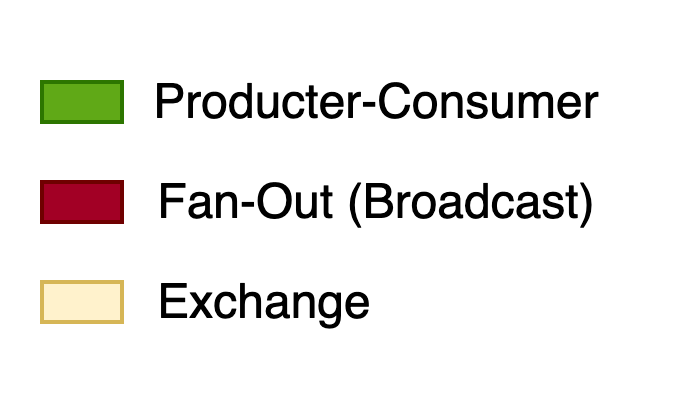
\includegraphics[width=0.30\linewidth]{colas.png}
\end{figure}
\end{itemize}
\begin{itemize}
    \item Las entidades que pueden ser escaladas a multiples unidades de computo se representan de la siguiente forma:
\begin{figure}[H]
\centering
    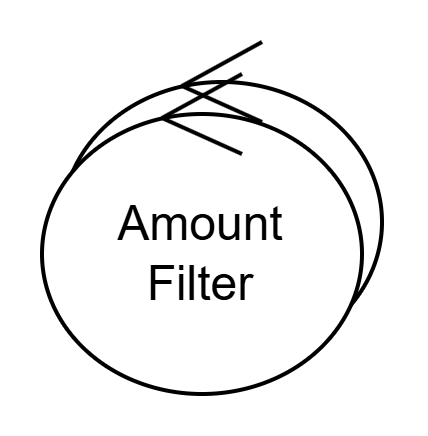
\includegraphics[width=0.15\linewidth]{multiple_computo.png}
\end{figure}
\end{itemize}

Cada worker tiene asociado una cola de input y una cola de output, salvo los aggregators que obtienen resultados de muchos workers en una unica cola y se encargan de agregar los resultados.

Las colas marcadas como tipo "broadcast" se basan en multiples colas producer-consumer, cada una de ellas conectadas a un worker de salida, el worker que se encarga de producir en esta cola iterara cada una de ellas dejando el mismo dato en todas, de esa forma cada worker de salida recibira el mismo mensaje y podra procesarlo de manera independiente. Usualmente usado para joiners.

Por otro lado el manejo de EOF (end of file) se realiza mediante un mensaje especial que indica a los workers que no habra mas datos a procesar. El request handler encola ese mensaje en todas las colas de entrada y los sucesivos workers iran propagando el mensaje de EOF a medida que terminan su trabajo, una vez que todos los EOF correspondientes lleguen a las colas de resultados entonces el Response Builder arma la respuesta y la envia al cliente indicando que una query ya fue completamente procesada

Todos los resultaados seran insertados en diferentes colas, una para cada consulta, el Response builder sera el encargado de leer de ellas y mandar una unica respuesta para la consulta correspondiente

A continuación, se muestran cuatro extractos del diagrama de robustez, destacando los aspectos más relevantes de cada consulta.

\subsection*{Consulta 1}
Es la más simple. Requiere tres filtros encadenados (\textbf{Year Filter}, \textbf{Hour Filter} y \textbf{Amount Filter}).  
Cada etapa puede escalarse mediante un esquema \textbf{producer--consumer}: los workers consumen mensajes de la cola, procesan la entrada y deciden si reenviarla a la cola de salidao descartarla.

\begin{figure}[H]
    \centering
    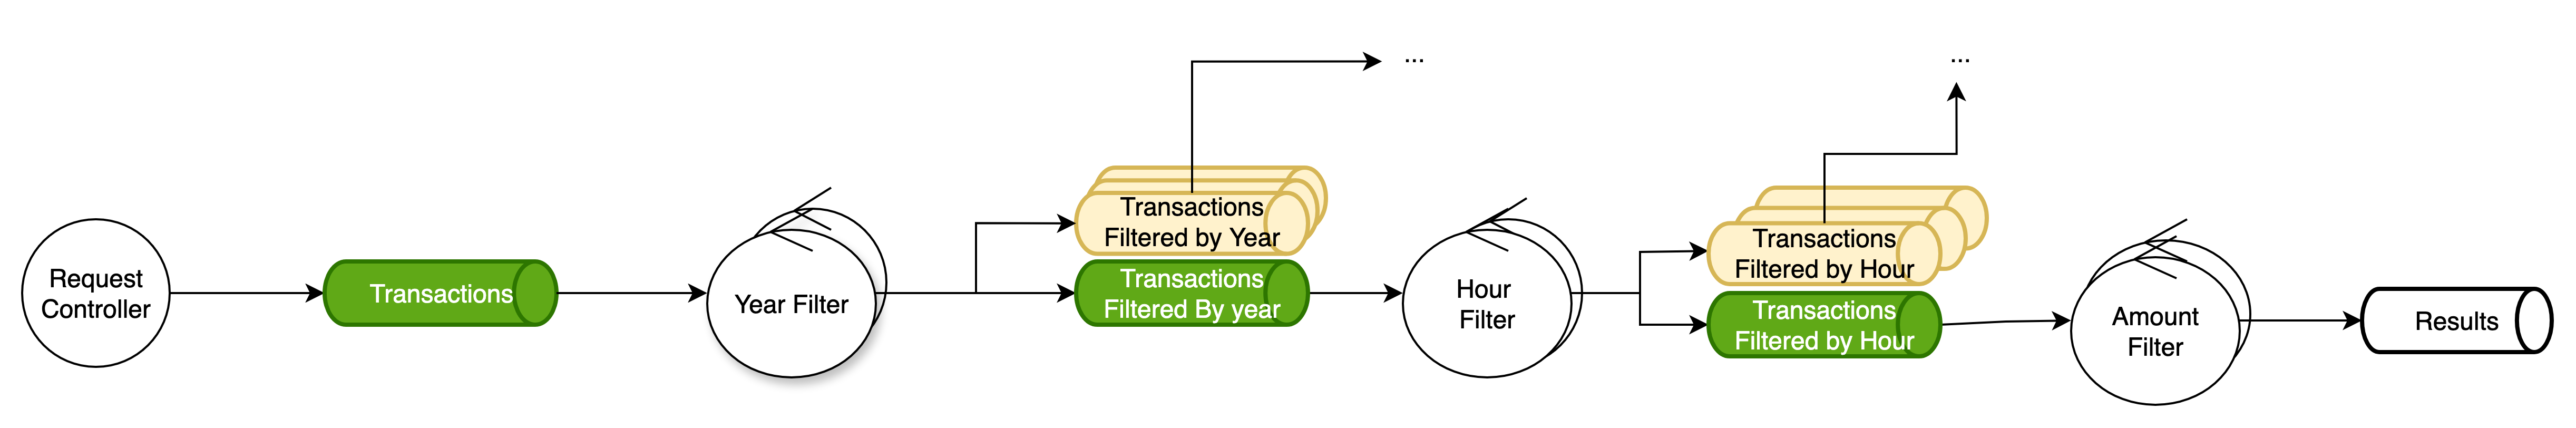
\includegraphics[width=1.0\textwidth]{consulta1.png}
    \caption{Diagrama de robustez - Consulta 1}
\end{figure}


\subsection*{Consulta 2}
Ya que al final es necesario hacer un join de dos datasets distintos, el joiner final procesara y guardara todos los datos de \texttt{Menu Items} antes de comenzar a procesar los datos de \texttt{Transactions profit and quantity}, ya que estos tardaran mucho mas en llegar.
\begin{enumerate}
    \item \textbf{Menu Items}: los datos se difunden a todos los \texttt{Item Id Joiner}. Estos almacenan en memoria la lista de ítems (pocos y estáticos) y luego consumen de la cola \textbf{Items with max values} (producer--consumer) para realizar los joins. Como el total de items del menú siempre son 8 entonces podemos cargarlos en memoria sin problemas. \newline
    \textbf{Transactions Items}: Estas colas obtienen los datos directo del request handler que es lo que recibe los datasets del cliente, no hay ningun pre-proceso previo asi que estos datos representan filas del dataset original.
    \item \textbf{Transactions 2024-2025}: Estas colas contienen las transacciones filtradas por año, ademas cada worker elimina las columnas que no van a ser necesarias en los proximos pasos de la query.
    \item \textbf{Transactions profit and quantity}: En este caso contenemos una unica cola que va a tener todos los resultados parciales de nuestros groupers segun la data que pudieron obtener de la cola anterior, en este caso el profit and quantity aggregator sera el encargado de agregar los resultados parciales de los groupers para tener los resultados finales
    \item \textbf{Items with max values}: Estas colas contienen las transacciones el resultado de agrupar todas las transacciones por mes con el profit y el quantity.
\end{enumerate}

\begin{figure}[H]
    \centering
    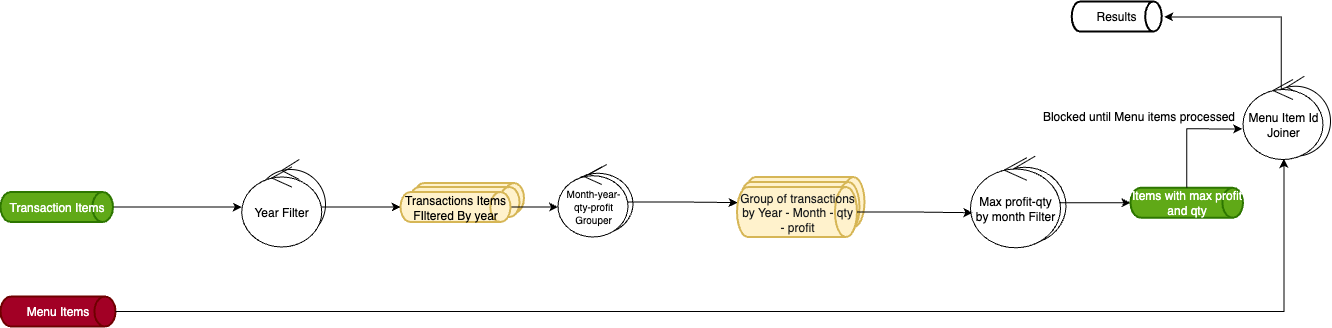
\includegraphics[width=1.0\textwidth]{consulta2.png}
    \caption{Diagrama de robustez - Consulta 2}
\end{figure}

\subsection*{Consulta 3}
\begin{enumerate}
    \item \textbf{Stores\_3}: Estos datos se difunden a todos los \texttt{Store ID Joiner} y contienen todos los registros de las tiendas. Estos almacenan en memoria la lista de ítems (pocos y estáticos) y luego consumen de la cola \textbf{Transactions per semester} (producer--consumer) para realizar los joins. Como el total de items del menú siempre son 10 entonces podemos cargarlos en memoria sin problemas. En este caso tiene el sufijo \_3 para diferenciarlo de las colas de la consulta 4.\newline
    \textbf{Transactions}: Estas colas contienen las transacciones originales sin ningun pre-proceso previo asi que estos datos representan filas del dataset original.
    \item \textbf{Transactions 2024-2025}: Estas colas contienen las transacciones filtradas por año, ademas cada worker elimina las columnas que no van a ser necesarias en los proximos pasos de la query.
    \item \textbf{Transactions 6 AM - 11 PM}: Estas colas contienen las transacciones filtradas por hora, ademas cada worker elimina las columnas que no van a ser necesarias en los proximos pasos de la query.
    \item \textbf{Transactions per semester}: Siguiendo la logica anterior tenemos un único aggregator que se encarga de obtener los datos parciales de los groupers y los agrega en un solo resultado final, el cual sera enviado a la cola de \textbf{Transactions with tpv}.
    \item \textbf{Transactions with tpv}: Estas colas contienen las transacciones ya agrupadas con el TPV calculado, listas para ser unidas con los datos de las sucursales.
\end{enumerate}

\begin{figure}[H]
    \centering
    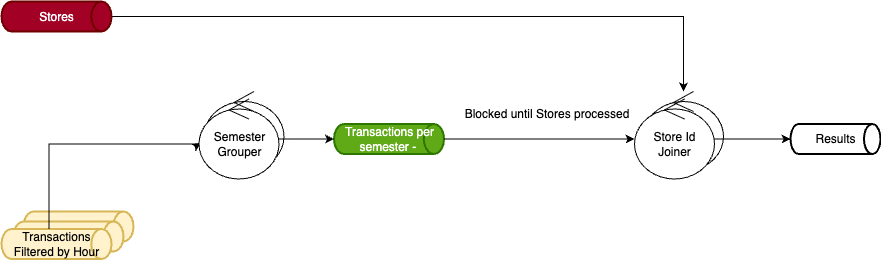
\includegraphics[width=1.0\textwidth]{consulta3.png}
    \caption{Diagrama de robustez - Consulta 3}
\end{figure}

\subsection*{Consulta 4}
\begin{itemize}
    \item \textbf{Stores\_4}: Estos datos se difunden a todos los \texttt{Store ID Joiner} y contienen todos los registros de las tiendas. Estos almacenan en memoria la lista de ítems (pocos y estáticos) y luego consumen de la cola \textbf{Transactions per semester} (producer--consumer) para realizar los joins. Como el total de items del menú siempre son 10 entonces podemos cargarlos en memoria sin problemas. En este caso tiene el sufijo \_4 para diferenciarlo de las colas de la consulta 3.\newline
    \textbf{Transactions}: Estas colas contienen las transacciones originales sin ningun pre-proceso previo asi que estos datos representan filas del dataset original.
    \textbf{Users}: Estas colas contienen los datos de los usuarios de las cafeterias, los cuales son pocos y estaticos, por lo que cada worker puede cargar todos los datos en memoria y realizar los joins de manera correcta.
    \item \textbf{Transactions 2024-2025}: Estas colas contienen las transacciones filtradas por año, ademas cada worker elimina las columnas que no van a ser necesarias en los proximos pasos de la query.
    \item \textbf{Transactions 6 AM - 11 PM}: Estas colas contienen las transacciones filtradas por hora, ademas cada worker elimina las columnas que no van a ser necesarias en los proximos pasos de la query.
    \item \textbf{Transactions with user and store}: Al igual que en los casos anteriores, tenemos un agregator que recibe los datos parciales de los groupers y los agrega en un solo resultado final, el cual sera enviado a la cola de \textbf{Top 3 transactions per store}.
    \item \textbf{Top 3 transactions per store}: Estas colas se comportan como si fuera un fan-out donde todos los resultados llegan a todos los workers, ya que estos resultados nunca son muy grandes (solo 3 resultados por cada sucursal) y al tenerlo en memoria, los workers pueden realizar los joins de manera correcta.
    \item \textbf{Top 3 transactions with birthday}: Estas colas contienen los resultados finales de la consulta, con los 3 clientes que más compras han hecho en cada sucursal, junto con su fecha de cumpleaños.
\end{itemize}


\begin{figure}[H]
    \centering
    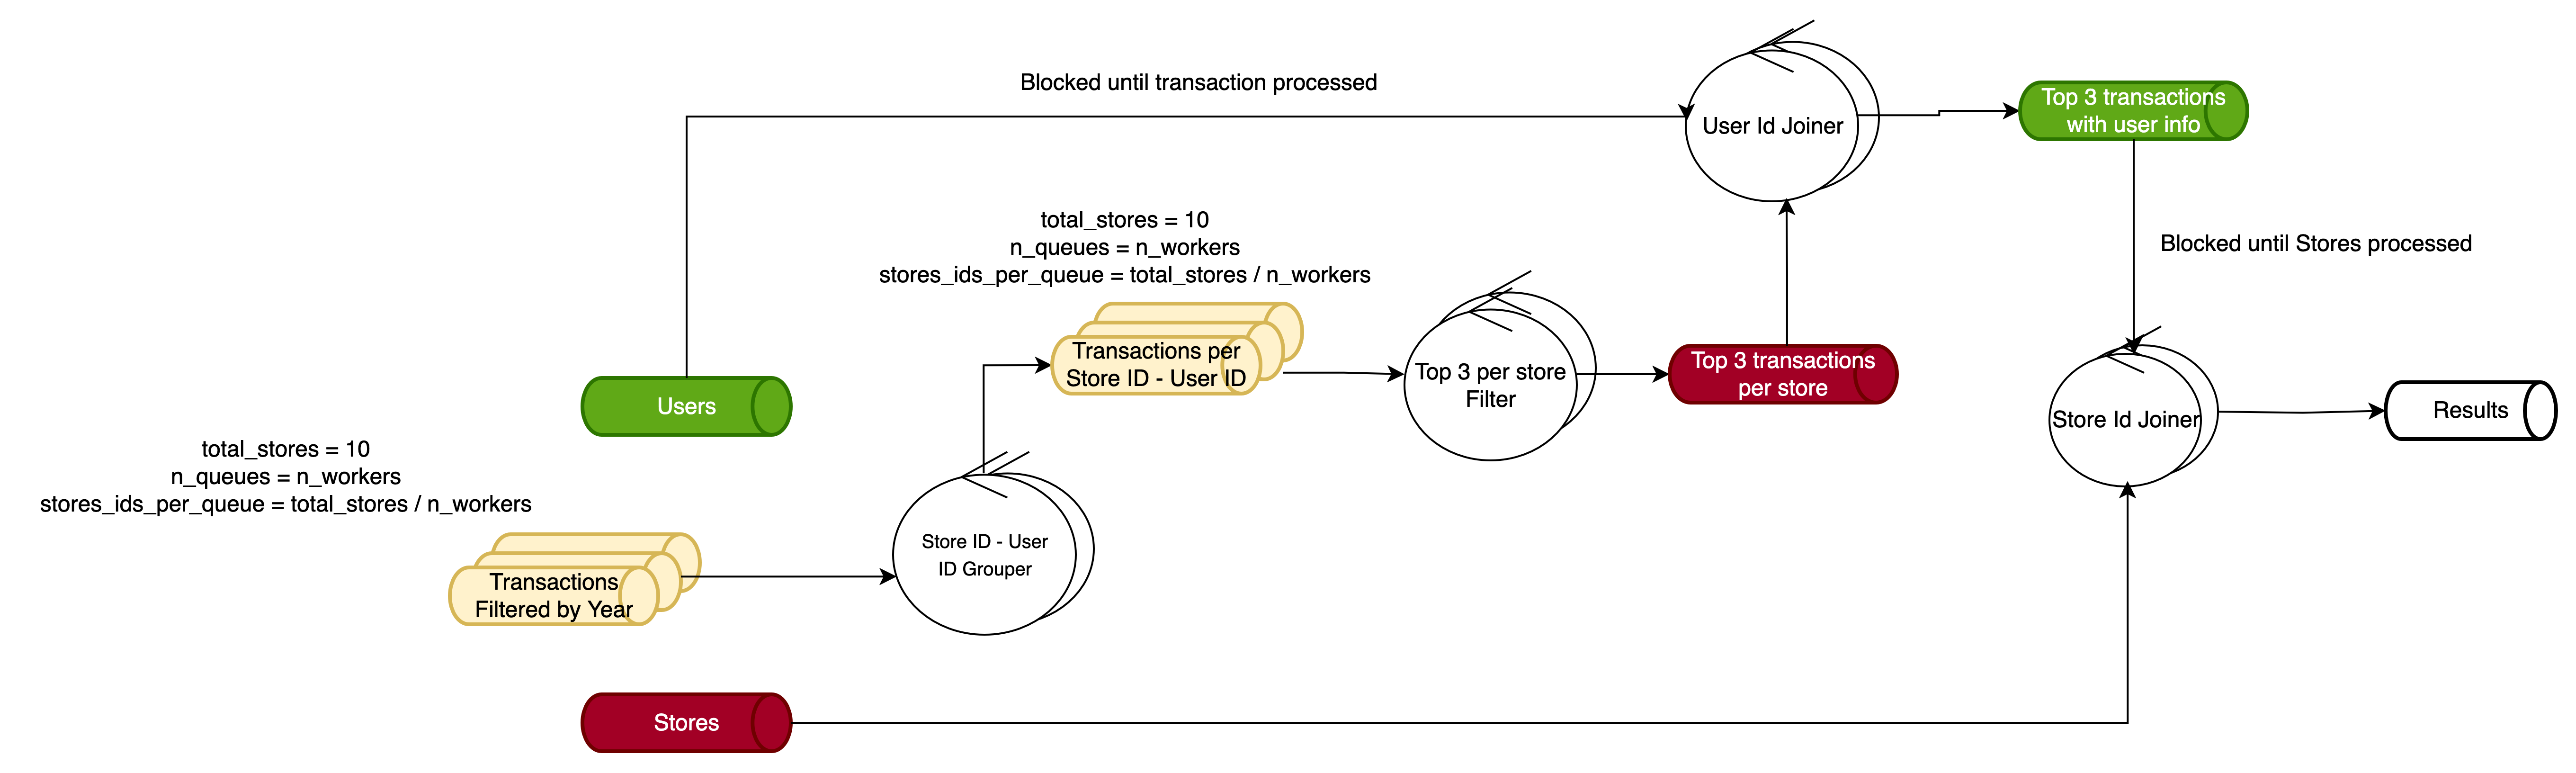
\includegraphics[width=1.0\textwidth]{consulta4.png}
    \caption{Diagrama de robustez - Consulta 4}
\end{figure}

\subsubsection{Diagrama de Despliegue}

Podemos ver como los toda comunicación interna es realizada mediante RabbitMQ (el middleware).
En este caso se agrupan los workers por tipo en un mismo nodo de computo.

\begin{figure}[H]
    \centering
    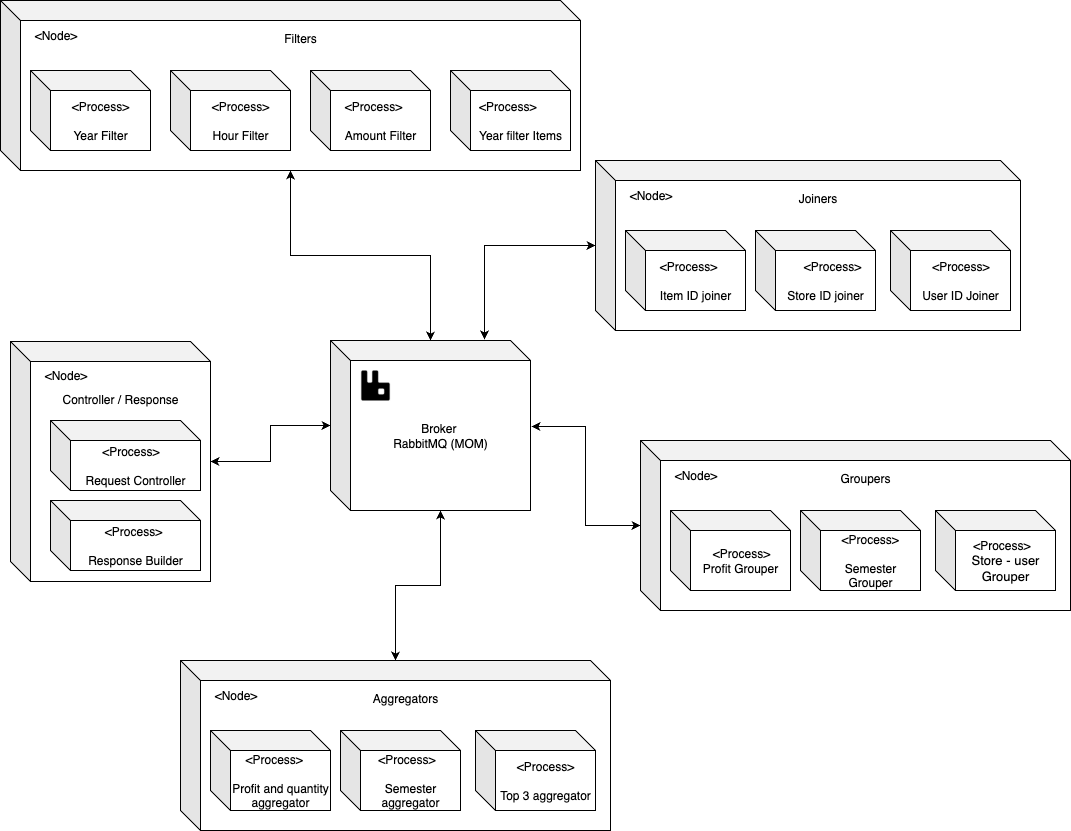
\includegraphics[width=1\linewidth]{despliegue.png}
\end{figure}


\subsection{Vista Lógica}
\subsubsection{DAG}
\begin{figure}[H]
\centering
    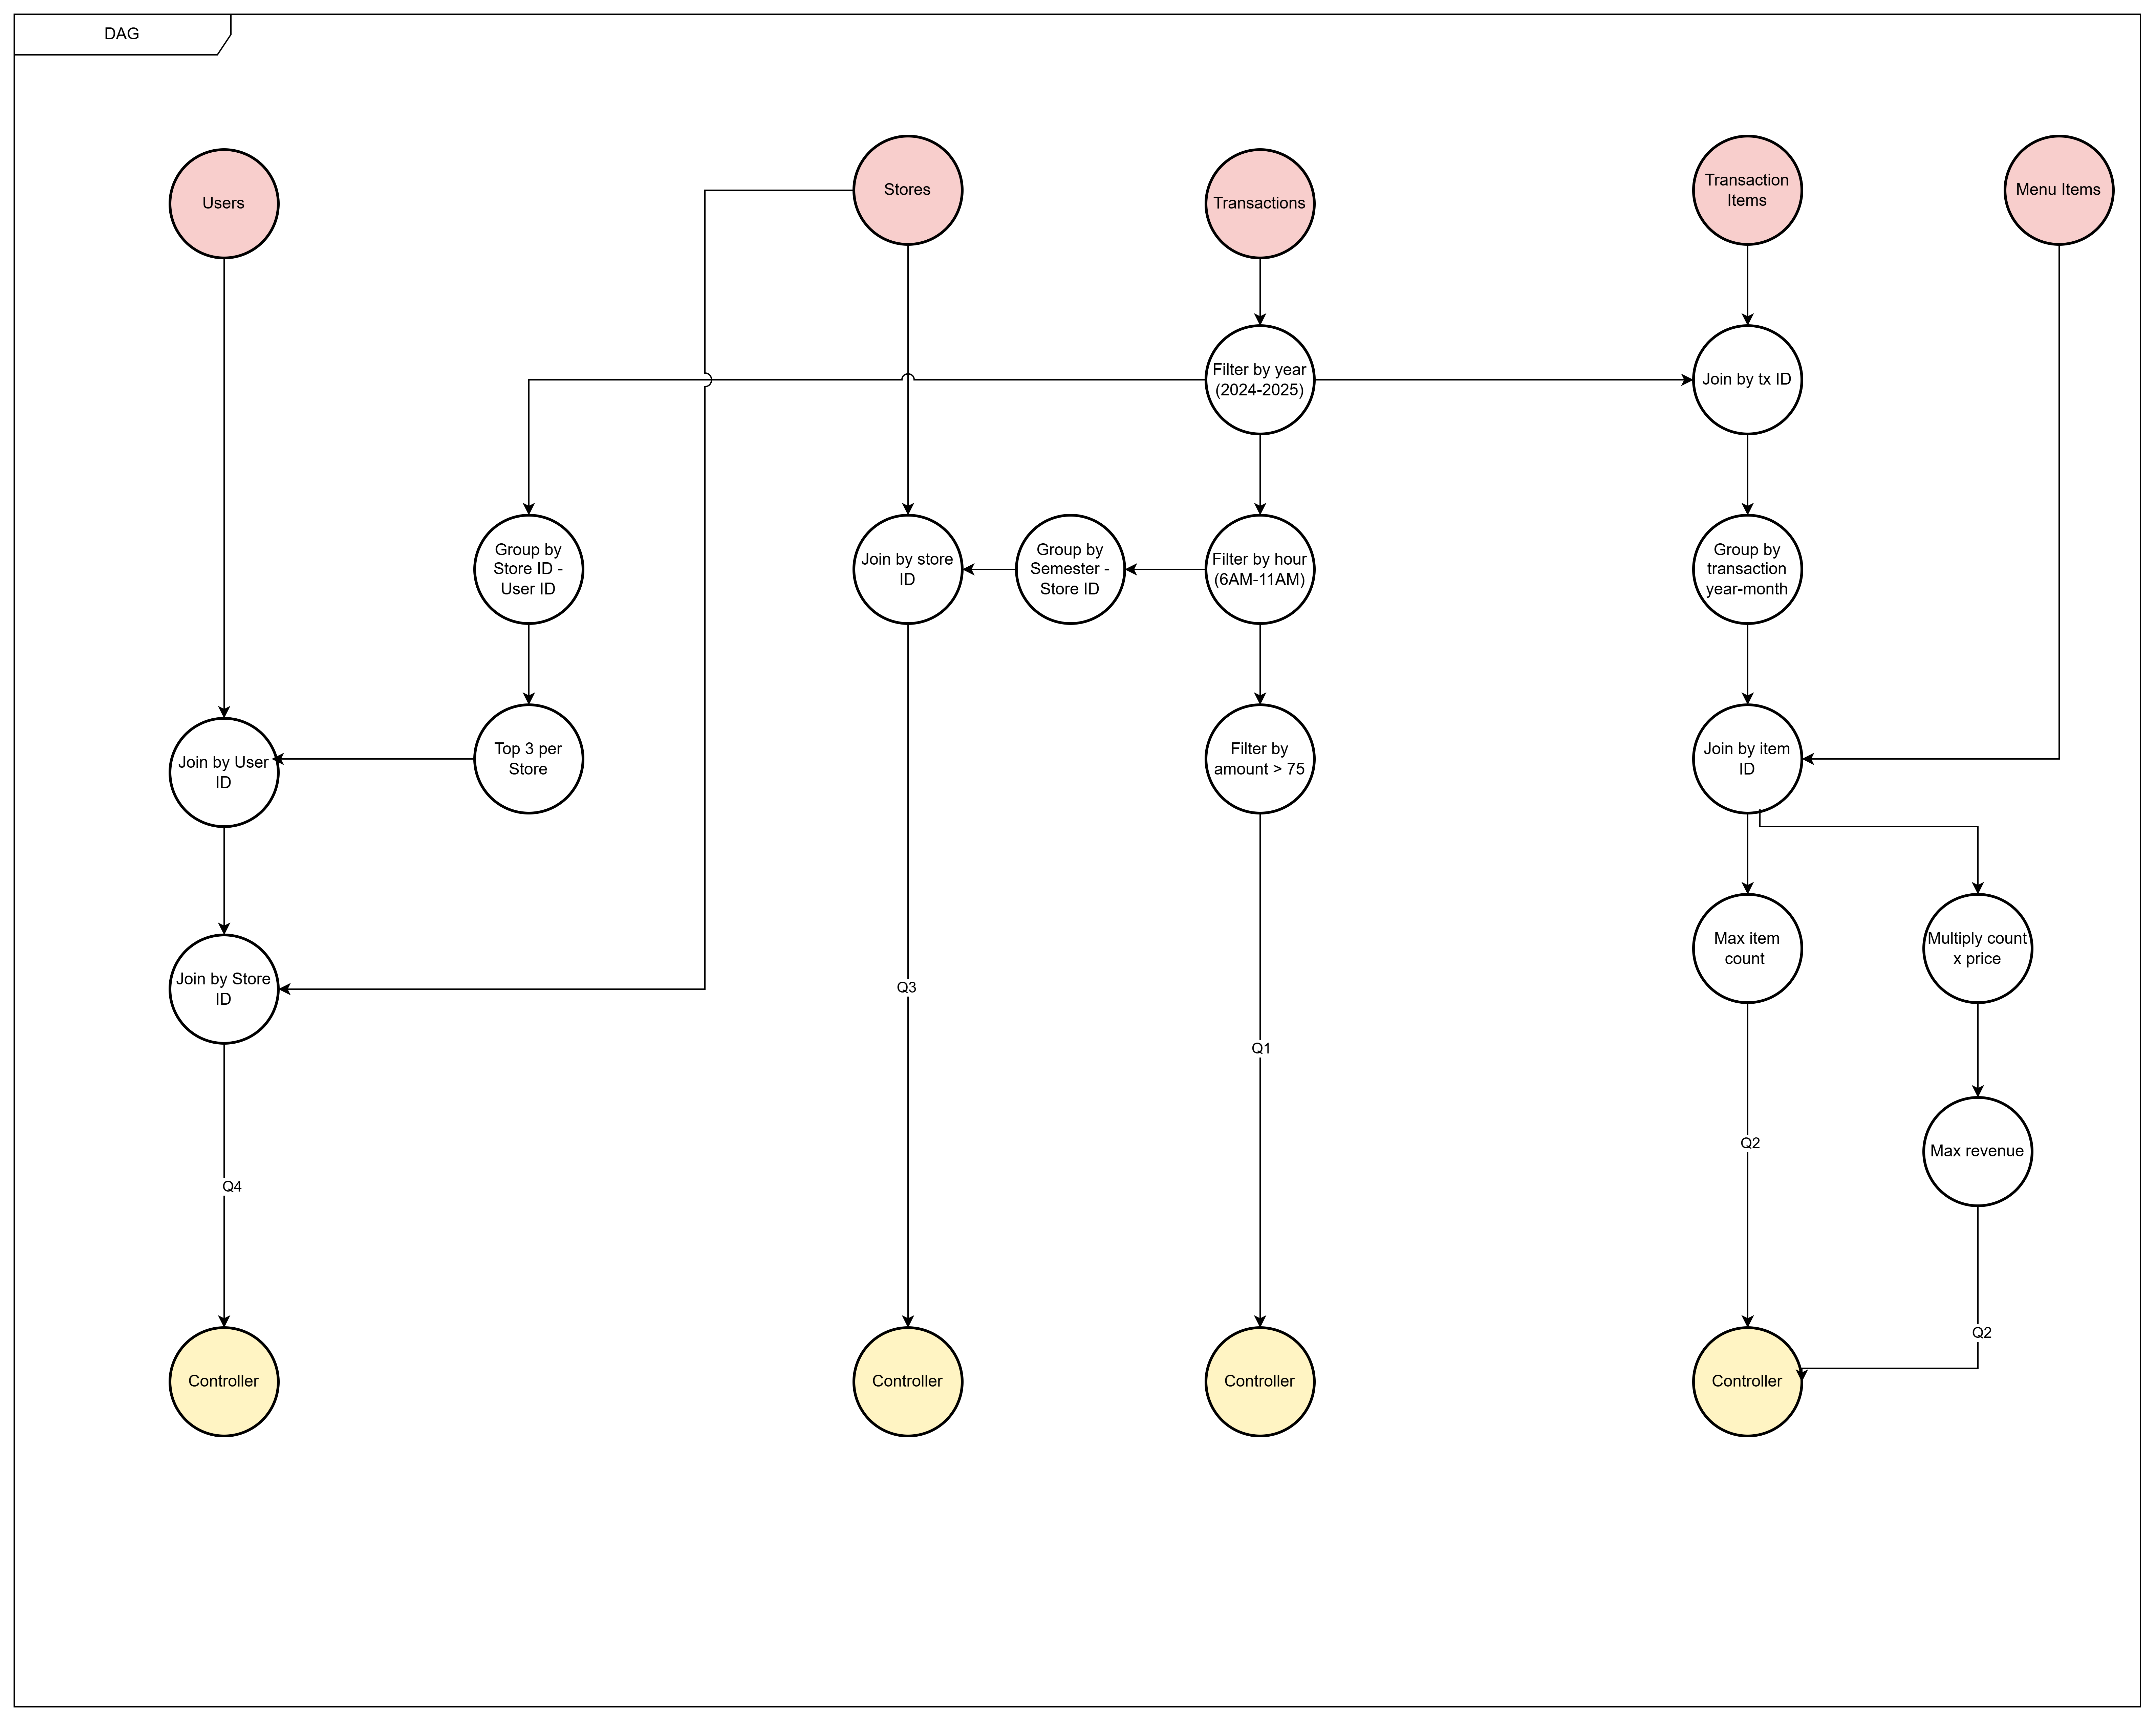
\includegraphics[width=1\linewidth]{DAG.png}
\end{figure}
Se visualiza un directed acyclic graph que muestra el flujo de datos siendo atravezado por los distintos componentes, comenzando de arriba hacia abajo. Los trabajadores (workers) se dividen en agrupadores (groupers), acumuladores (joiners), agregadores (aggregators) y filtradores (filters). Las fuentes de información inicial, y donde se almacena finalmente lo procesado son a nivel de implementación colas.
Los aggregators son los nodos encargados de obtener data de los groupers y acumularla en un solo resultado final segun sea necesario, de esta manera los groupers pueden recibir cualquier tipo de data y agrupar en ba\textbf{}se a los datos que le lleguen.


\subsection{Vista de Desarrollo}
Aquí podemos visualizar como esta planeada la arquitectura del sistema desde la perspectiva del código. Se divide el sistema en distintos modulos para Client, Worker, Request Handler, Response builder y Middleware.

\subsubsection{Diagrama de Paquetes}
Se muestran los distintos modulos a implementar:\newline

El cliente tiene la responsabilidad de comunicarse con el Request handler para enviarle toda la data necesaria para procesar las 4 queries. Tiene como entrypoint un modulo main que se encarga de parsear la configuracion y comenzar la comunicacion llamando al modulo client. El serializer es un modulo con algunas funciones auxiliares que sirven para serializar y deserializar los paquetes a mandar
\begin{figure}[H]
    \centering
    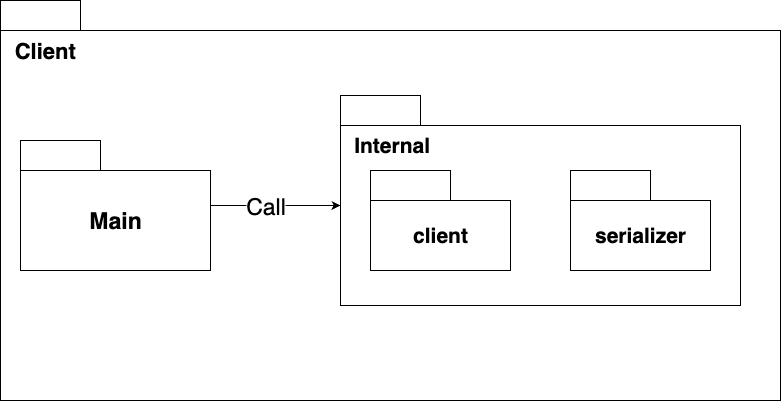
\includegraphics[width=0.8\linewidth]{paquete-client.png}
\end{figure}

Los workers tienen la tarea de filtrar, acumular o agrupar los diversos tipos de datos que lean de las colas a las que estes subscriptos. En este caso todos los tipos de workers comparten el mismo modulo main donde se parsea la configuracion y se inicializa el worker llamando al modulo worker, dicho modulo tiene la logica comun a todos los tipos de workers, como la conexion a RabbitMQ y el manejo de colas segun esten configuradas. Este modulo luego llamara a los modulos correspondientes segun el tipo de worker que sea donde ya se implemenara la lógica especifica para cada uno de ellos.
Para simplificacion del gráfico no se muestran todos los tipos de workers pero existe un modulo distinto para cada uno de ellos dentro de su respectivo paquete.
\begin{figure}[H]
    \centering
    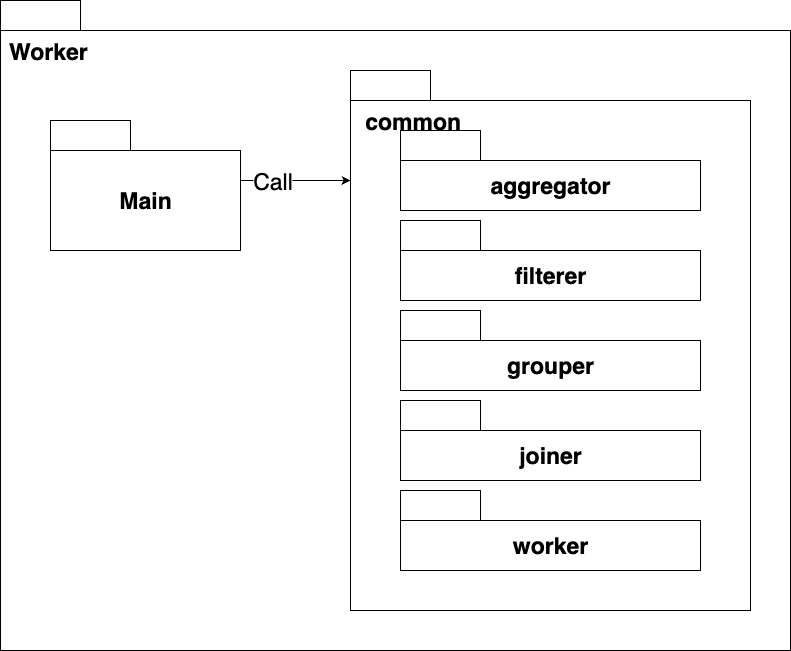
\includegraphics[width=0.8\linewidth]{paquete-worker.png}
\end{figure}

La tarea del request handler es interpretar los mensajes del cliente, para poder derivarlos a las diferentes colas de RabbitMQ. Tiene un modulo main que se encarga de parsear la configuracion y comenzar la comunicacion llamando al modulo request handler, el cual tiene la logica para interpretar los mensajes del cliente y enviarlos a las colas correspondientes para empezar el trabajo.
\begin{figure}[H]
    \centering
    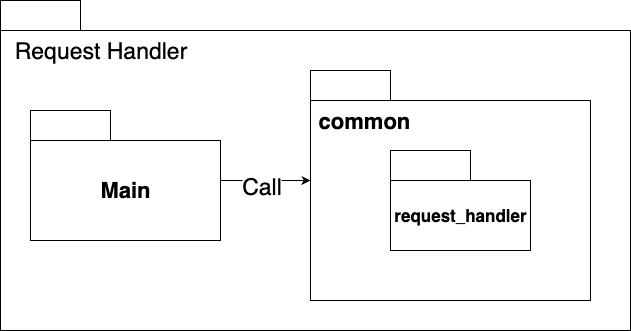
\includegraphics[width=0.8\linewidth]{paquete-rh.png}
\end{figure}

El Middleware es el que se encarga principalmente de la interaccion con la libreria de RabbitMQ. Contiene un modulo con la interfaz (provista a traves del enunciado). La implementacion de dicha interfaz se encuentra en el modulo middleware, el cual tiene la logica para conectarse a RabbitMQ, encolar y desencolar mensajes. El modulo de utils contiene funciones auxiliares utilizadas por el modulo middleware.
\begin{figure}[H]
    \centering
    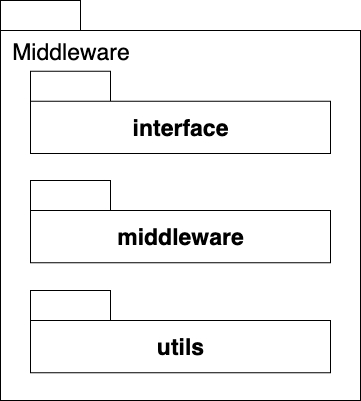
\includegraphics[width=0.8\linewidth]{paquete-middleware.png}
\end{figure}

El response builder tiene la responsabilidad de procesar los resultados parciales de cada query que van llegando de los ultimos workers y armar la respuesta final para enviarsela al request handler, quien luego se encargara de enviarla al cliente. Tiene un modulo main que se encarga de parsear la configuracion y comenzar la comunicacion llamando al modulo response builder, el cual tiene la logica para leer los resultados parciales de las colas correspondientes y armar la respuesta final.
\begin{figure}[H]
    \centering
    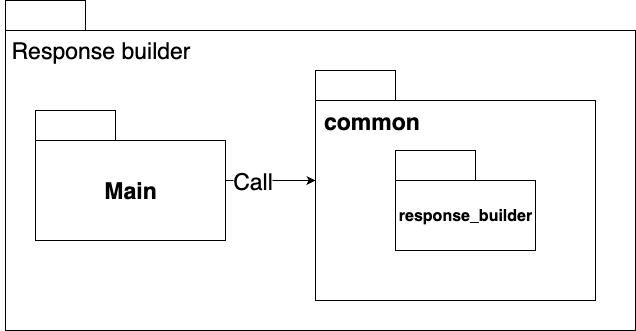
\includegraphics[width=0.8\linewidth]{paquete-rb.png}
\end{figure}

\subsection{Vista de Procesos}

\paragraph{Se representa la interacción entre los componentes del sistema, su forma de comunicación de principio a fin. Es posible visualizar la concurrencia del sistema, asi como también la escalabilidad y distribuición de tareas.}

\subsubsection{Diagrama de Actividad}
\paragraph{En el siguiente diagrama se muestra parcialmente el proceso de obtener los productos más vendidos y que más ganancias han generado, para cada mes, en este caso se representa solamente la parte de mayor complejidad de obtención, la de mayor valor y no solo mayor cantidad de ventas.}
\paragraph{*Se considera más complejo debido a que los pasos necesarios para obtener este dato es superior a la de calcular el producto más vendido en cantidad.}
\begin{figure}[H]
    \centering
    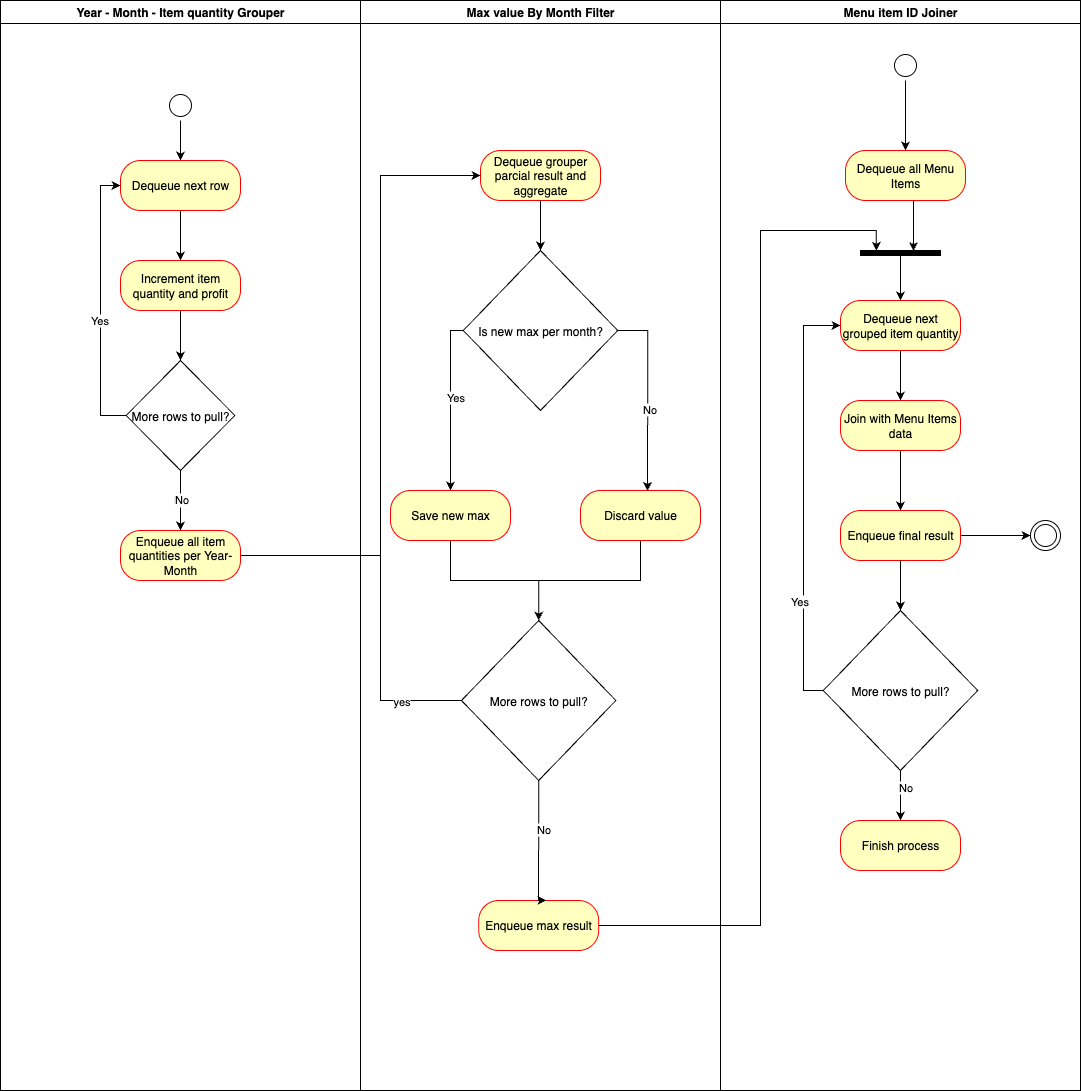
\includegraphics[width=1\linewidth]{actividades.png}
\end{figure}
\paragraph{El proceso que observamos en el diagrama comienza con los groupers, en este caso estos tomaran la data de diferentes colas de entrada donde tienen transacciones e iran sumando los valores correspondiente a un item del menu en un mismo año y mes, para luego enviar sus resultados a la cola de salida para que el aggregator los pueda procesar}
\paragraph{El aggregator se encargara de recibir todos los resultados parciales de los groupers y sumarlos en un solo resultado final para cada año-mes. Este sera enviado a la cola de salida para que el joiner del menu de items pueda agregar el nombre del item a los resultados}
\paragraph{El joiner del menu de items en un principio espera a obtener los datos del dataset de menu items ya que sin estos no podra realizar el join, una vez los tiene se queda esperando por el resultado del aggregator. Une vez recibidos los resultados finales del aggregator y realizar el join con los datos correctos envia dicha fila de resultado a la cola de resultados que va a ser leida por el response builder }

\paragraph{Manejo de EOF:}En el siguiente diagrama se muestra como se maneja el EOF desde que comienza una query hasta que termina para determinar cuando los workers dejan de esperar por datos y dejan de leer una cola. Para simplificar el diagrama se muestran solo algunos filtros del total ya que el proceso es el mismo para todos.
\begin{figure}[H]
    \centering
    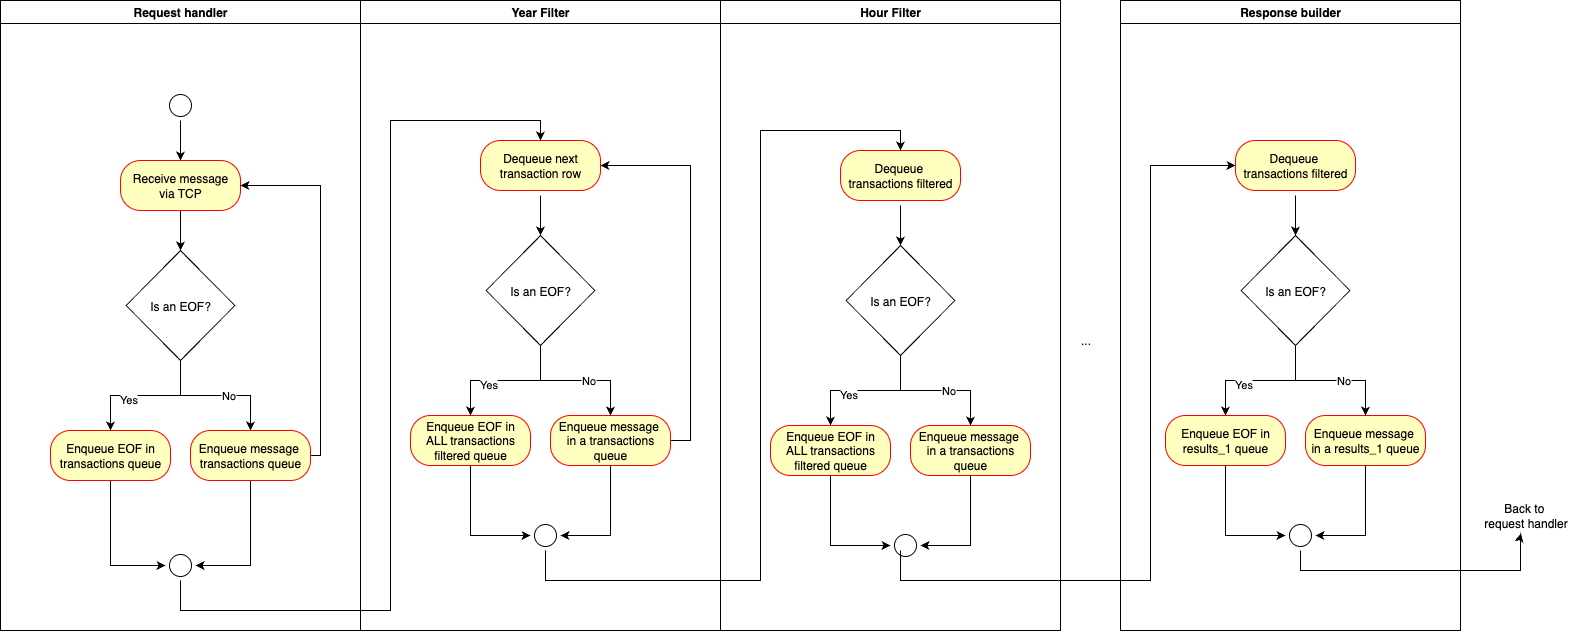
\includegraphics[width=1\linewidth]{actividades-eof.png}
\end{figure}
\paragraph{Este proceso se da como en una especie de cascada. En primer lugar el cliente enviara datos indicando que tipo de dataset esta enviando \(transactions, menu_items, etc.\) mandando un EOF cuando ya envio todos los datos relacionados a un tipo especifico. El request handler detectara este mensaje de EOF y encolara un nuevo mensaje EOF en las colas de salida correspondientes. Asi se dara el proceso donde cada vez que un worker lee un mensaje de EOF debe propagarlo hacia la cola de salida sea cual sea, asi se asegura de que el proximo worker tambien lo recibe. Una vez llega al ultimo worker de la query este encola el resultado final indicando tambien que ha terminado de procesar todos los datos. El response builder espera a recibir todos los EOFs de todos los workers de salida para saber que ya tiene la totalidad de la respuesta para la query entonces puede procesarla y enviarla al request handler.}

\subsubsection{Diagrama de Secuencia}

\begin{figure}[H]
    \centering
    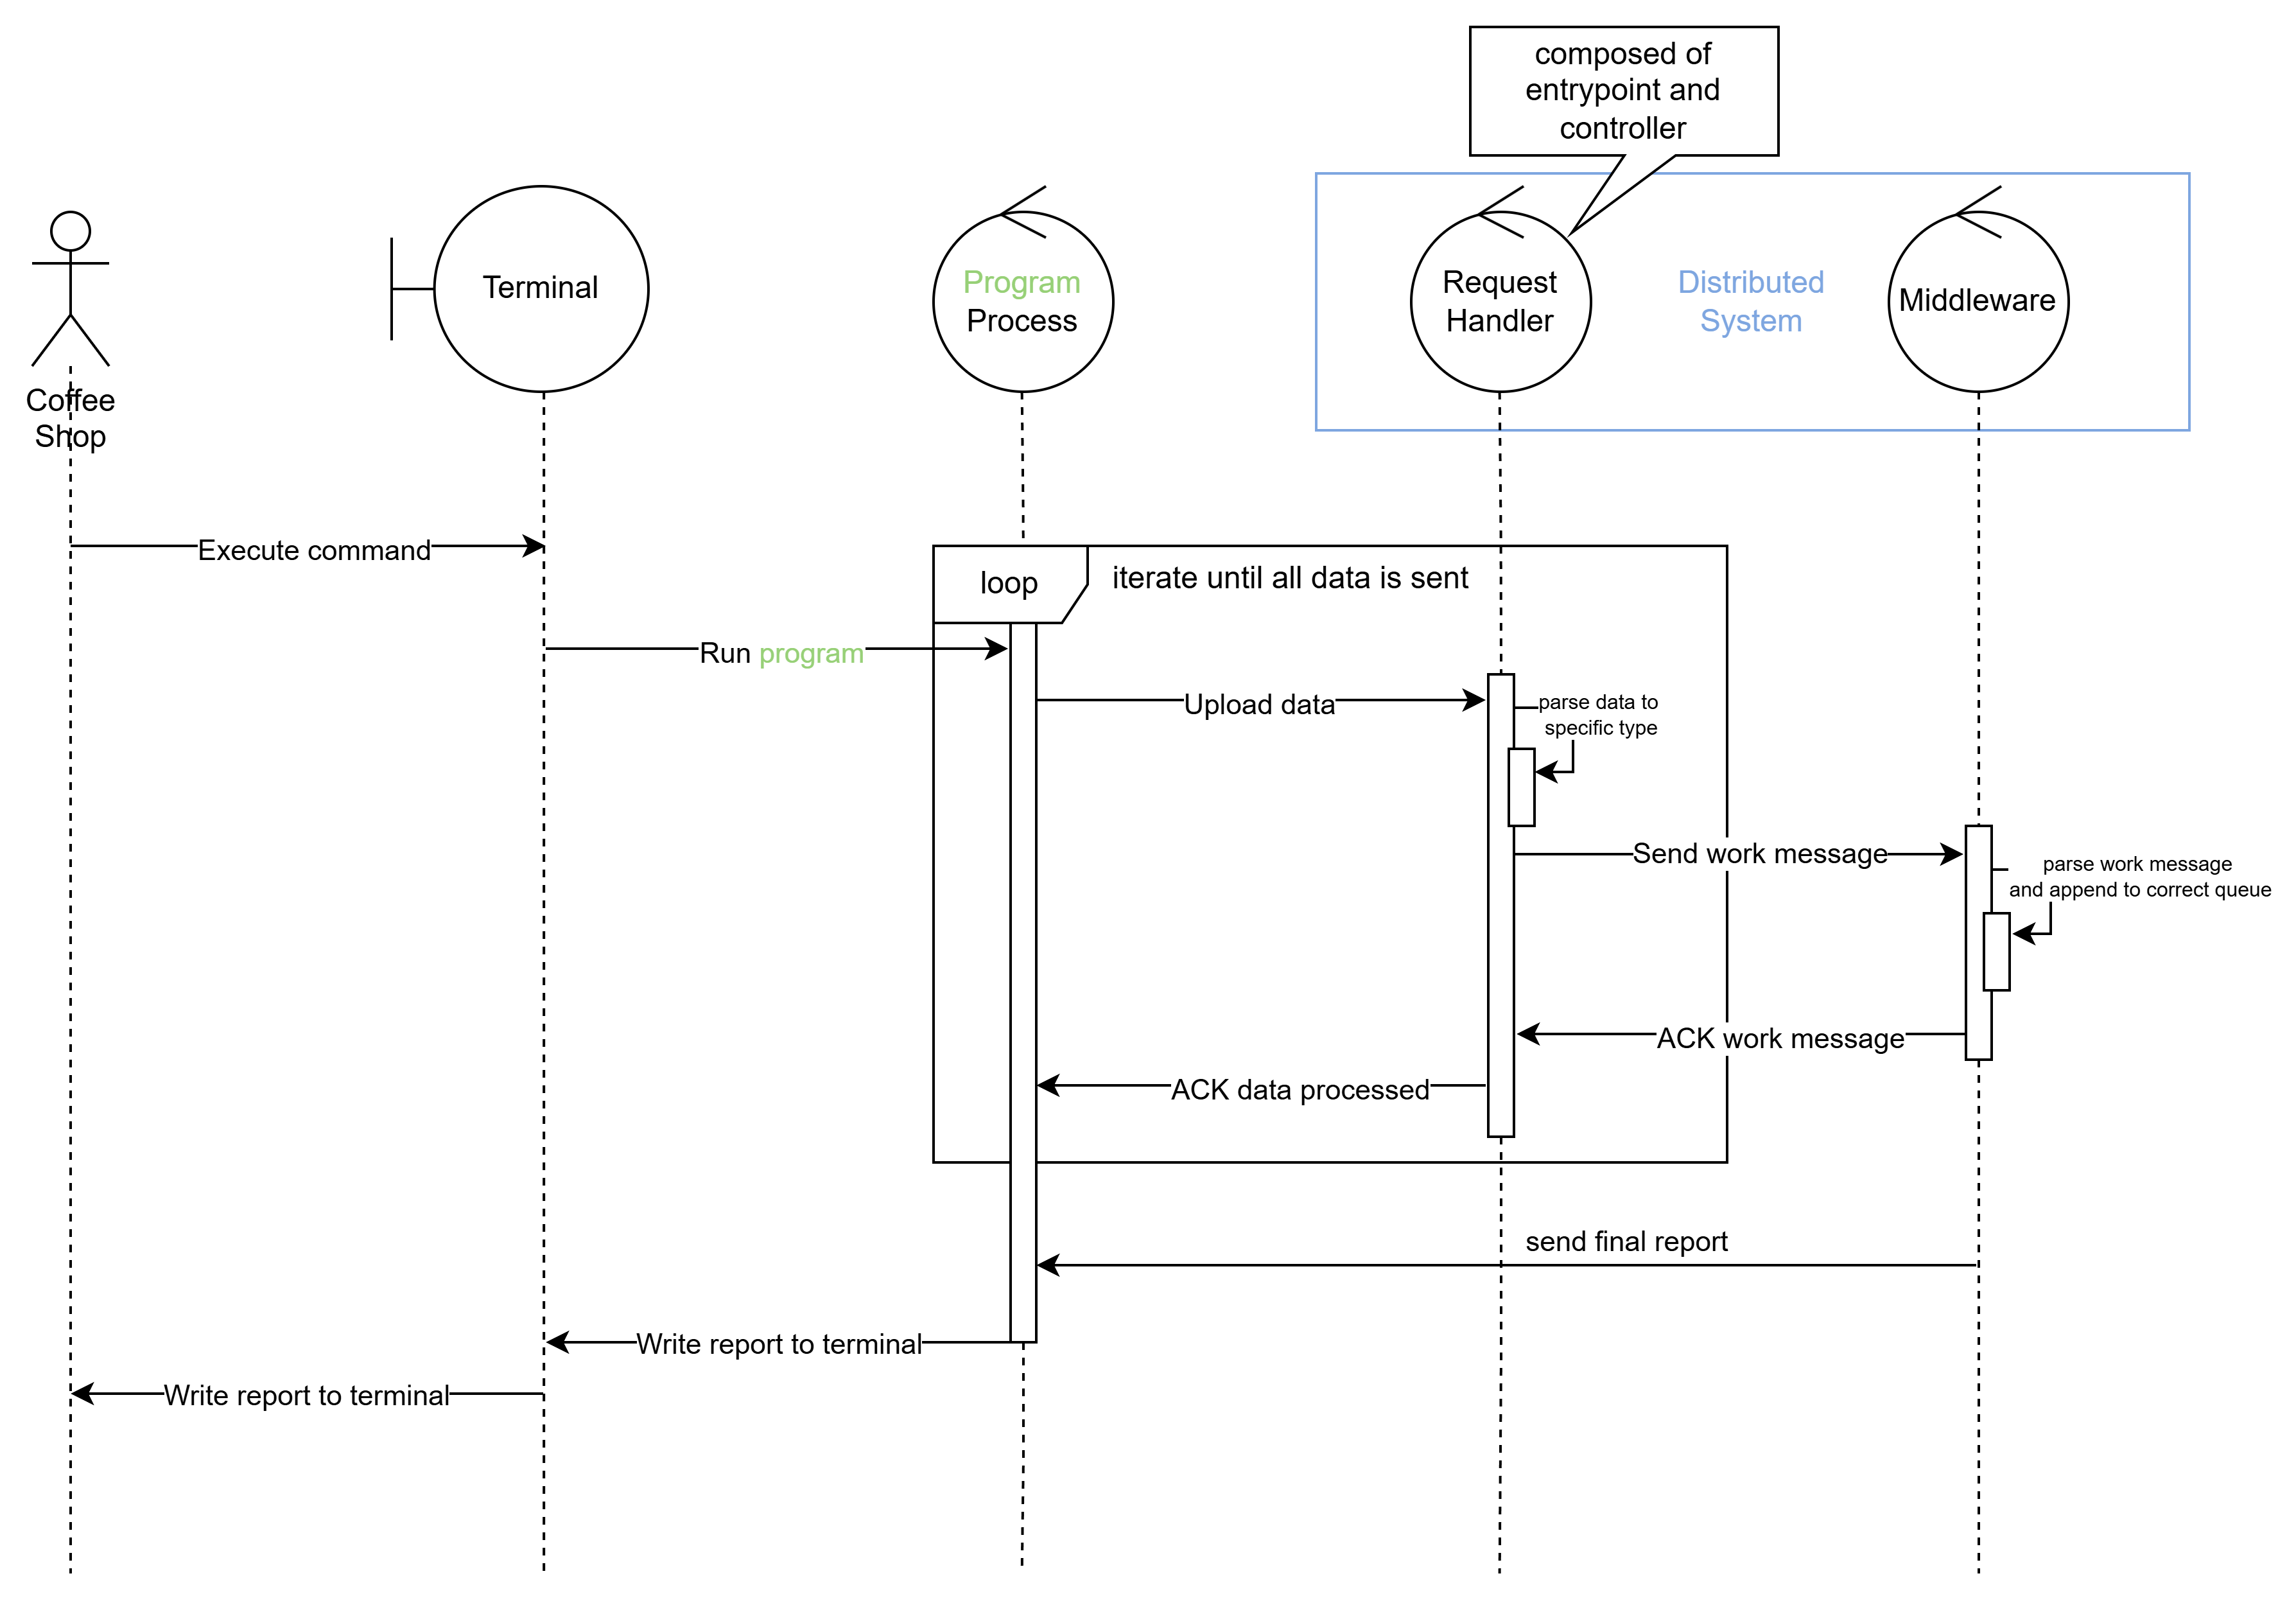
\includegraphics[width=0.8\linewidth]{secuencia.png}
\end{figure}
\paragraph{Podemos ver como el cliente desde la terminal inicializa el programa, el cual establece conexión con el sistema mediante el Request Handler. La comunicación entre ellos consistira en enviar todos los datos necesarios en bucle, cada mensaje transmitido por el cliente incluye un header informando el tipo de archivo transmitido, el tamaño del payload, y un bit que indica si hay datos pendientes por transmitir posteriores a ese mensaje. Una vez que ya no haya nada más que enviar, el Middleware le enviará el programa el resultado final, el cual sera mostrado por terminal al usuario.}

\section{Comunicacion}\label{sec:comunicacion}

\subsection{Vista general}
\paragraph{Se describe el protocolo de comunicación utilizado entre el client y request_handler para la transferencia de archivos CSV y la obtención de resultados. El protocolo utiliza framing de tipo TLV (type-lenght-value) para prevenir short reads/writes.}


\subsection{Sistema de Tipos de Archivo}

El protocolo utiliza un sistema de enumeración (\texttt{enum}) para los tipos de archivo, con el fin de asegurar que tanto el cliente como el servidor estén de acuerdo en la categorización de los datos:

\begin{lstlisting}[language=Go]
	type FileType int
	
	const (
	FileTypeTransactions      FileType = 0  // Datos de transacciones
	FileTypeTransactionItems  FileType = 1  // Detalles de los ítems de transacción
	FileTypeStores            FileType = 2  // Información de tiendas
	FileTypeMenuItems         FileType = 3  // Catálogo de ítems del menú
	FileTypeUsers             FileType = 4  // Información de usuarios
	)
\end{lstlisting}

\subsection*{Estructura de Directorios}

El cliente espera la siguiente estructura de directorios bajo \texttt{/data}:

\begin{lstlisting}
	/data/
	├── transactions/         → FileType 0 (FileTypeTransactions)
	│   ├── file1.csv
	│   └── file2.csv
	├── transaction_items/    → FileType 1 (FileTypeTransactionItems)
	│   ├── file1.csv
	│   └── file2.csv
	├── stores/               → FileType 2 (FileTypeStores)
	│   ├── file1.csv
	│   └── file2.csv
	├── menu_items/           → FileType 3 (FileTypeMenuItems)
	│   ├── file1.csv
	│   └── file2.csv
	└── users/                → FileType 4 (FileTypeUsers)
	├── file1.csv
	└── file2.csv
\end{lstlisting}

\section{Tipos de Mensaje}

Todos los mensajes comienzan con un byte identificador del tipo de mensaje:

\begin{longtable}{|l|c|c|p{7cm}|}
	\hline
	\textbf{Tipo de Mensaje} & \textbf{Valor} & \textbf{Dirección} & \textbf{Descripción} \\
	\hline
	MessageTypeBatch & 0x01 & Cliente → Servidor & Lote de datos CSV \\
	\hline
	MessageTypeEOF & 0x02 & Cliente → Servidor & Fin de un tipo de archivo \\
	\hline
	MessageTypeFinalEOF & 0x03 & Cliente → Servidor & Todos los datos transferidos \\
	\hline
	MessageTypeACK & 0x04 & Servidor → Cliente & Confirmación de recepción (ACK) \\
	\hline
	MessageTypeResultChunk & 0x05 & Servidor → Cliente & Fragmento de datos de resultado \\
	\hline
	MessageTypeResultEOF & 0x06 & Servidor → Cliente & Fin del resultado \\
	\hline
\end{longtable}

\section{Formatos de Mensaje}

\subsection{Batch Message (0x01)}

Transfiere un lote de datos CSV con metadatos.

\textbf{Formato:}
\begin{lstlisting}[basicstyle=\ttfamily\scriptsize,breaklines=true]
	┌─────────┬──────────┬──────────┬─────────────┬─────────────┬──────────┬─────────┐
	│ Tipo    │ Size   │ TipoArchivo │ ChunkActual │ TotalChunks │ NumFilas │ Payload │
	│ (1 byte)│ (4 bytes)│ (1 byte)   │ (4 bytes)   │ (4 bytes)   │ (4 bytes)│ Variable │
	└─────────┴──────────┴──────────┴─────────────┴─────────────┴──────────┴─────────┘
\end{lstlisting}

\textbf{Campos:}
\begin{itemize}
	\item \textbf{Tipo}: 0x01
	\item \textbf{Tamaño de Marco (Frame Size)}: Tamaño total del marco (excluyendo el byte de tipo) — \textit{uint32 Big Endian}
	\item \textbf{TipoArchivo}: Valor del tipo de archivo (0–4) — 1 byte
	\item \textbf{ChunkActual}: Número del fragmento actual (indexado desde 1) — \textit{uint32 Big Endian}
	\item \textbf{TotalChunks}: Número total de fragmentos — \textit{uint32 Big Endian}
	\item \textbf{NumFilas}: Número de filas CSV en este fragmento — \textit{uint32 Big Endian}
	\item \textbf{Payload}: Filas CSV separadas por saltos de línea — longitud variable
\end{itemize}

\subsection{Mensaje EOF (0x02)}

Indica la finalización de todos los archivos para un tipo de archivo específico.

\textbf{Campos:}
\begin{itemize}
	\item \textbf{Tipo}: 0x02
	\item \textbf{TipoArchivo}: Valor del tipo de archivo (0–4)
\end{itemize}

\subsection{Mensaje Final EOF (0x03)}

Indica que la transferencia de todos los datos ha finalizado para todos los tipos de archivo.

\subsection{Mensaje ACK (0x04)}

Confirma la recepción exitosa de un mensaje.

\subsection{Mensaje de resultado parcial (0x05)}

Transfiere un fragmento de datos de resultado desde el servidor hacia el cliente.

\textbf{Campos:}
\begin{itemize}
	\item \textbf{Tipo}: 0x05
	\item \textbf{QueueID}: Identificador de cola de resultados (1–4) — \textit{uint32 Big Endian}
	\item \textbf{ChunkActual}: Número de fragmento actual — \textit{uint32 Big Endian}
	\item \textbf{TotalChunks}: Número total de fragmentos para este resultado — \textit{uint32 Big Endian}
	\item \textbf{DataLen}: Longitud de los datos — \textit{uint32 Big Endian}
	\item \textbf{Data}: Datos binarios del resultado — longitud variable
\end{itemize}

\subsection{Mensaje Result EOF (0x06)}

Indica el final de los resultados provenientes de una cola específica.

\textbf{Campos:}
\begin{itemize}
	\item \textbf{Tipo}: 0x06
	\item \textbf{QueueID}: Identificador de cola de resultados — \textit{uint32 Big Endian}
\end{itemize}

\subsection{Implementación multicliente}

\paragraph{Para la implementación de soporte de multiples clientes en simultaneo, se hicieron modificaciones a los mensajes que envia el cliente al request\_handler. Todo mensaje de datos enviado (es decir, contenido de un archivo csv), contiene un header delimitado por un caracter newline. Este header de una sola columna informa el ID de cliente que envia el mensaje.}

\paragraph{Luego, la comunicación interna del sistema propaga este header de principio a fin, de esta forma, todo tipo de worker al recibir un mensaje analiza el cliente de origen para el mensaje, y lo almacena o procesa de forma acorde.}

\paragraph{Finalmente, el response\_builder interpreta también los resultados específicos de cada cliente y los deriva a la cola de resultados correspondiente, el request\_handler, los consume, y mediante la conexión TCP establecida en el inicio envia los resultados, tal y como se hacia con la implementación de un único cliente.}
\end{document}
